\section {Análisis espacial}

Los datos obtenidos mediante el simulador del proceso evolutivo, contienen información que nos
permiten analizarlos en el contexto de un SIG, para identificar los focos de infestación mediante
técnicas de interpolación espacial.

Los niveles de riesgos fueron determinados de acuerdo a los tipos de zonas determinados en la
\secref{subsec:cap4-zonificacion}. Se consideran de mayor riesgo las zonas propicias para el
desarrollo del Aedes aegypti. En la \tabref{tab:niveles-riesgo-zonas}, se presentan los niveles de
riesgo definidos según la \tabref{tab:cap4-puntaje-zona}.


\begin{table}[!hptb]
    \begin{minipage}{\textwidth}
\begin{center}
    \caption{\label{tab:niveles-riesgo-zonas} Niveles de infestación de las zonas.}
    \begin{tabular}{p{3cm} l c c c}
        \hline \\
         Niveles de  & Color & Mínimo$^a$ & Máximo$^a$ \\
         infestación & identificador & $u(x,y)$   & $u(x,y)$  \\
        \hline
        \hline\\
        Muy bajo  & \cellcolor{muybajo}& 0  & 19 \\
        Bajo    & \cellcolor{bajo}& 20 & 35 \\
        Normal & \cellcolor{normal}& 36 & 51 \\
        Alto   & \cellcolor{alto}& 52 & 69 \\
        Muy Alto & \cellcolor{muyalto} & 70 & --$^b$\\
    \end{tabular}
    \footnotetext[1]{Rango mínimo y máximo de $u(x,y)$ permitido para el tipo de zona.}
    \footnotetext[2]{No se estableció un límite superior para este nivel. }
\end{center}
    \end{minipage}
\end{table}

La distribución geográfica, dispersión y niveles de infestación de las poblaciones de Aedes aegypti
son presentadas como mapas de interpolación, donde para la interpolación espacial fueron
seleccionados los individuos pertenecientes a las poblaciones correspondientes a un día del
periodo de simulación.

\begin{figure}[!htbp]
    \centering
    \begin{subfigure}[b]{0.45\textwidth}
            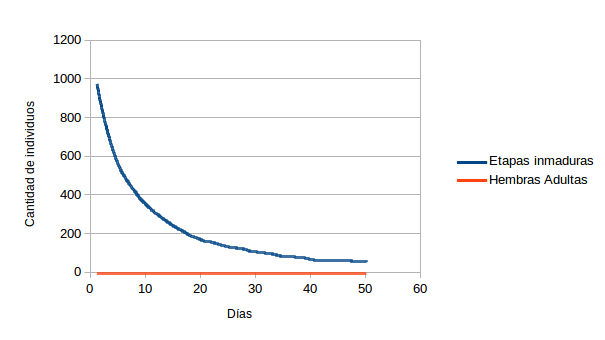
\includegraphics[width=\textwidth]{capitulo-6/graphics/desarrollo-poblacion-15.png}
            \caption{\label{fig:desarrollo-poblacion-15}Población a 15 \textcelsius.}
    \end{subfigure}
    ~~~~
    \begin{subfigure}[b]{0.45\textwidth}
            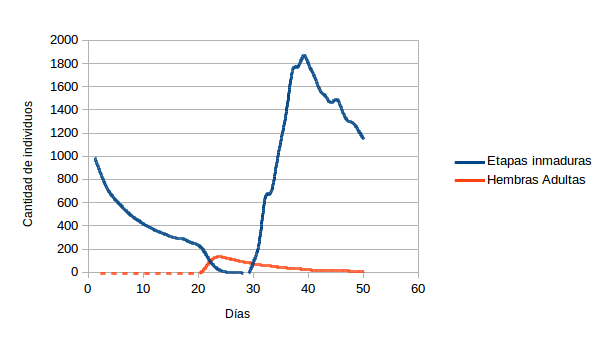
\includegraphics[width=\textwidth]{capitulo-6/graphics/desarrollo-poblacion-20.png}
            \caption{\label{fig:desarrollo-poblacion-20}Población a 20 \textcelsius.}
    \end{subfigure}

    \begin{subfigure}[b]{0.45\textwidth}
            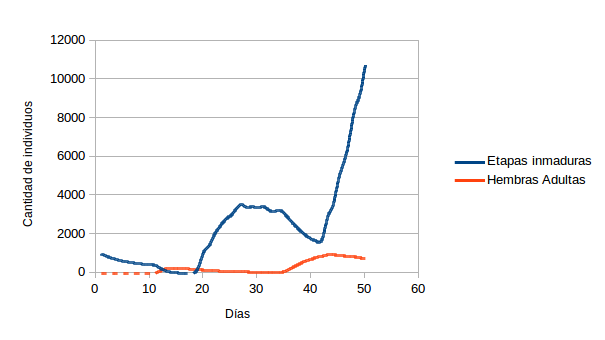
\includegraphics[width=\textwidth]{capitulo-6/graphics/desarrollo-poblacion-24.png}
            \caption{\label{fig:desarrollo-poblacion-24}Población a 24 \textcelsius.}
    \end{subfigure}
    ~~~~
    \begin{subfigure}[b]{0.45\textwidth}
            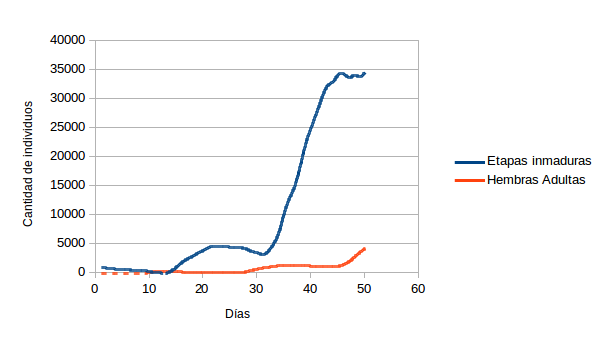
\includegraphics[width=\textwidth]{capitulo-6/graphics/desarrollo-poblacion-27.png}
            \caption{\label{fig:desarrollo-poblacion-27}Población a 27 \textcelsius.}
    \end{subfigure}

    \begin{subfigure}[b]{0.45\textwidth}
            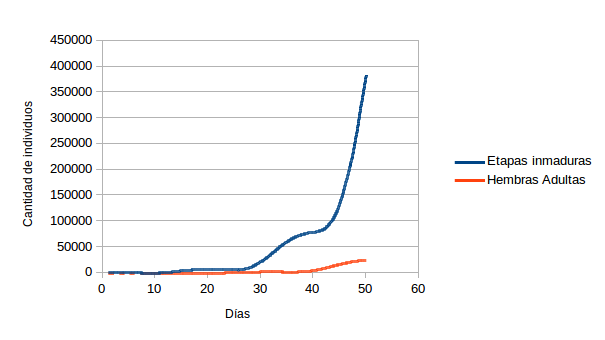
\includegraphics[width=\textwidth]{capitulo-6/graphics/desarrollo-poblacion-30.png}
            \caption{\label{fig:desarrollo-poblacion-30}Población a 30 \textcelsius.}
    \end{subfigure}
    ~~~~
    \begin{subfigure}[b]{0.45\textwidth}
            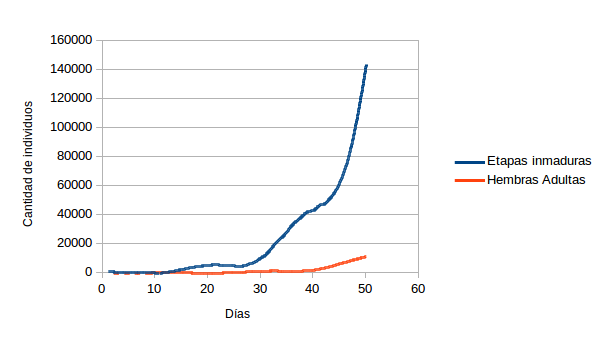
\includegraphics[width=\textwidth]{capitulo-6/graphics/desarrollo-poblacion-34.png}
            \caption{\label{fig:desarrollo-poblacion-34}Población a 34 \textcelsius.}
    \end{subfigure}

    \caption{\label{fig:desarrollo-poblacion-all} Análisis del comportamiento de la población de mosquitos en relación al tiempo a 6 temperaturas constantes (15-34 \textcelsius).}
\end{figure}

En la \figref{fig:desarrollo-poblacion-15}, se puede apreciar que el tamaño de la población a 15
\textcelsius, tiende a disminuir con el transcurrir del tiempo. Considerando que el estado inicial
de los individuos, para la simulación del proceso evolutivo, es el de larva, tenemos una tasa de
desarrollo igual a $44,33$ días de desarrollo
(\tabref{tab:desarrollo-larva-rueda1990temperature-test}), para las larvas. En un periodo de 50
días a 15 \textcelsius, no se pueden observar mosquitos adultos motivo por el cual la población
tiende a disminuir su tamaño y por ende el riesgo de infestación del área de estudio. En la
\figref{fig:niveles-infestacion-15} se puede observar el rápido decrecimiento de la población y de
los niveles de infestación. Para el octavo día, en la \figref{fig:niveles-infestacion-15-c}, se
puede apreciar el rápido decrecimiento en los niveles de infestación, debido a la disminución de
la población observados en \figref{fig:desarrollo-poblacion-15}. A partir del décimo día,
\figref{fig:niveles-infestacion-15-d}, los niveles de infestación se mantienen constantemente
bajos, por lo que los mapas de interpolación se mantienen constantes hasta el final del periodo de
simulación.

\begin{figure}[!htbp]
    \centering
    \begin{subfigure}[b]{0.45\textwidth}
            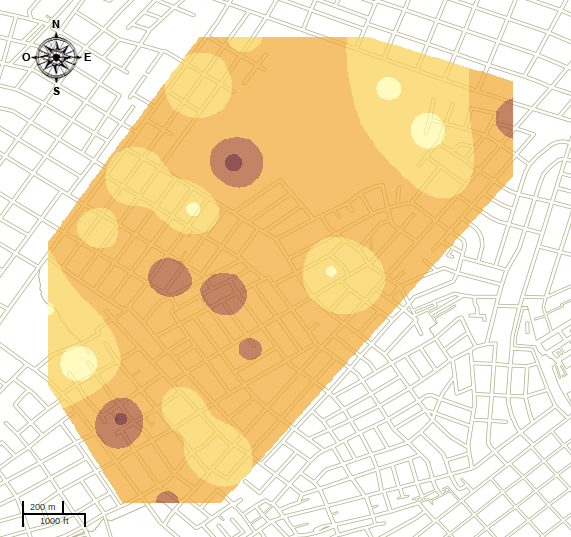
\includegraphics[width=\textwidth]{capitulo-6/graphics/raster/temp-15-0.png}
            \caption{\label{fig:niveles-infestacion-15-a}Primer día de simulación.}
    \end{subfigure}
    ~~
    \begin{subfigure}[b]{0.45\textwidth}
            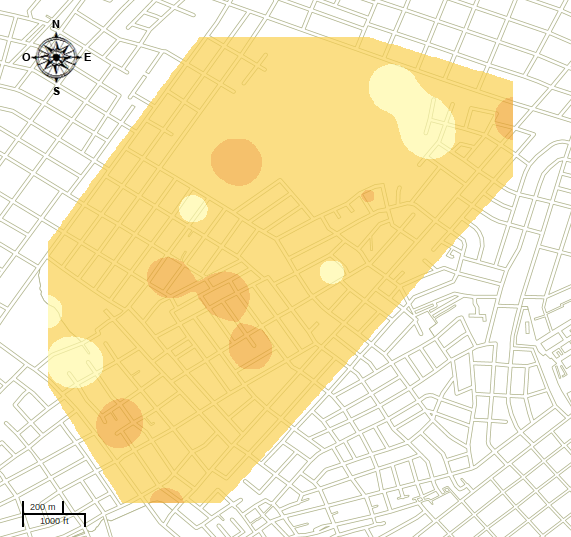
\includegraphics[width=\textwidth]{capitulo-6/graphics/raster/temp-15-2.png}
            \caption{\label{fig:niveles-infestacion-15-b}Día número 3 de simulación.}
    \end{subfigure}

    \begin{subfigure}[b]{0.45\textwidth}
            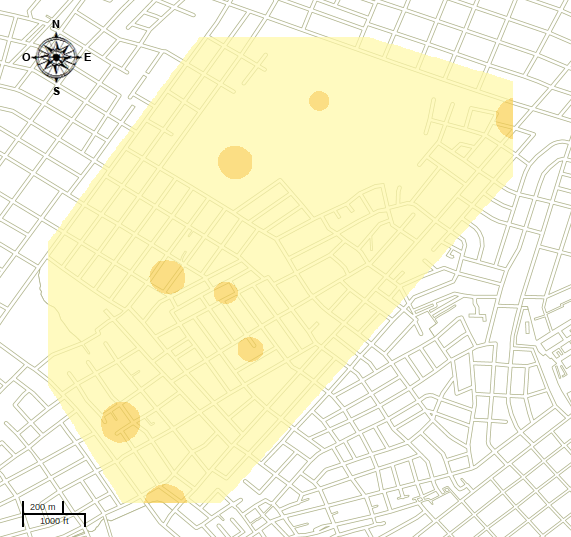
\includegraphics[width=\textwidth]{capitulo-6/graphics/raster/temp-15-7.png}
            \caption{\label{fig:niveles-infestacion-15-c}Día número 8 de simulación.}
    \end{subfigure}
    ~~
    \begin{subfigure}[b]{0.45\textwidth}
            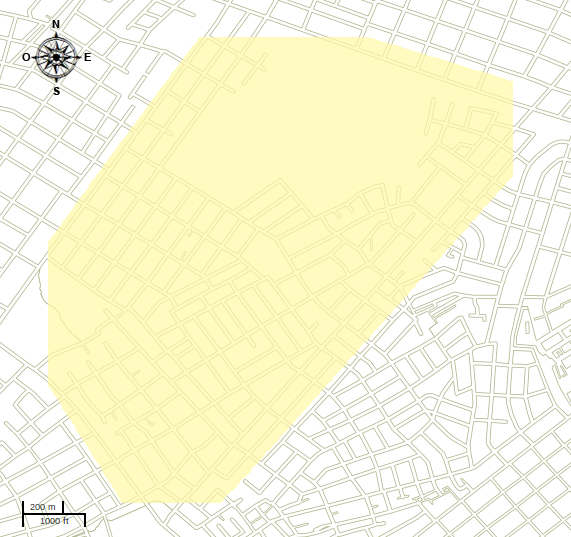
\includegraphics[width=\textwidth]{capitulo-6/graphics/raster/temp-15-9.png}
            \caption{\label{fig:niveles-infestacion-15-d}Día número 10 de simulación.}
    \end{subfigure}

    \caption{\label{fig:niveles-infestacion-15} Mapas de interpolación de la población correspondientes a los días 1, 3, 8 y 10 de simulación a 15 \textcelsius.}
\end{figure}


En la \figref{fig:desarrollo-poblacion-20}, se puede observar el comportamiento de la población a
20 \textcelsius, en donde la población de individuos en sus etapas inmaduras va decreciendo hasta
desaparecer temporalmente el día 28, no así la población de adultos. En la
\figref{fig:niveles-infestacion-20-b}, se puede observar que no existen mosquitos en sus etapas
inmaduras, para generar un mapa de interpolación del área, sin embargo se pueden observar la
distribución geográfica de las hembras adultas. Desde el día 21, en la
\figref{fig:desarrollo-poblacion-20}, comienzan a observarse los primeros mosquitos adultos, que a
partir del día 30, las hembras adultas, comienzan oviponer, generando la reaparición de la
población de mosquitos que alcanza su máximo valor en el día 39. En la
\figref{fig:niveles-infestacion-20} se puede apreciar los niveles de infestación para los
días 1, 28, 36 y 38 del periodo de simulación. Además se observa el desplazamiento de los focos de
infestación, causado por la dispersión de los adultos, que pasan de su estado inicial
(\figref{fig:niveles-infestacion-20-a}), a generar nuevos focos
(\figref{fig:niveles-infestacion-20-c} y \figref{fig:niveles-infestacion-20-d}). Cabe resaltar
que, un aumento en el tamaño de la población no necesariamente implica mayores niveles de
infestación. Esto se puede observar realizando una comparación entre los niveles de infestación
presentados en las \figref{fig:niveles-infestacion-20-c} y \figref{fig:niveles-infestacion-20-d},
y el tamaño de la población para los días 36 y 39 del periodo de simulación, en donde el día 39
cuenta con una población de mayor tamaño que el día 36, pero en este último se observan mayores
niveles de infestación. Esto se debe a que los mapas de interpolación dependen de la distribución
geográfica de los individuos de la población y la concentración de los mismos en $(x,y)$.


\begin{figure}[!htbp]
    \centering
    \begin{subfigure}[b]{0.45\textwidth}
            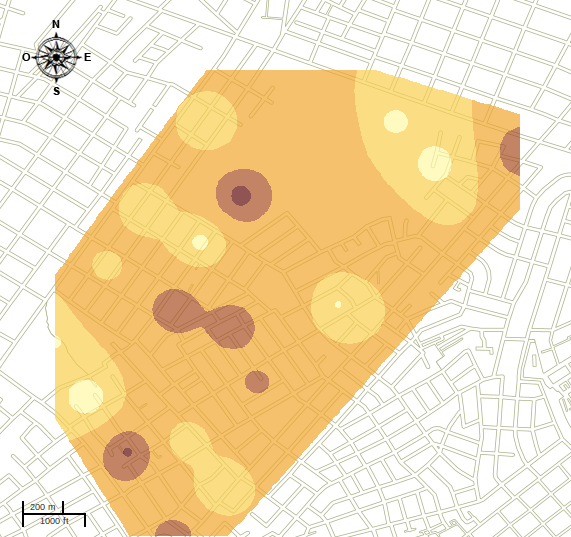
\includegraphics[width=\textwidth]{capitulo-6/graphics/raster/temp-20-0.png}
            \caption{\label{fig:niveles-infestacion-20-a}Primer día de simulación.}
    \end{subfigure}
    ~~
    \begin{subfigure}[b]{0.45\textwidth}
            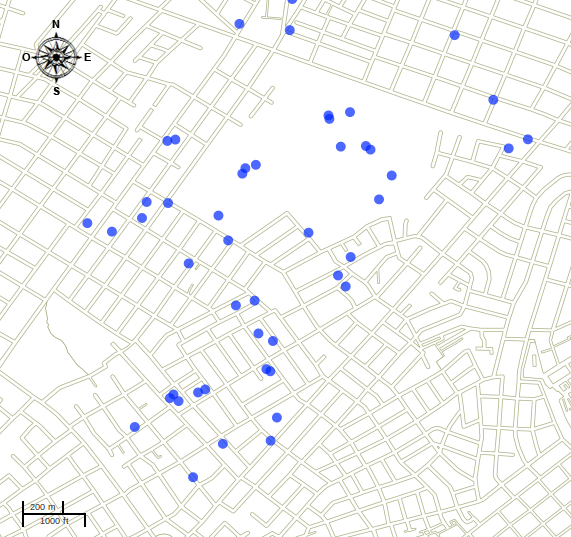
\includegraphics[width=\textwidth]{capitulo-6/graphics/raster/temp-20-28.png}
            \caption{\label{fig:niveles-infestacion-20-b}Día número 28 de simulación.}
    \end{subfigure}

    \begin{subfigure}[b]{0.45\textwidth}
            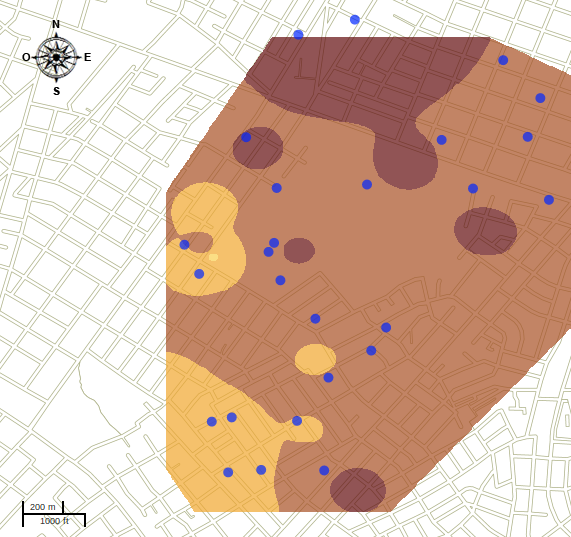
\includegraphics[width=\textwidth]{capitulo-6/graphics/raster/temp-20-35.png}
            \caption{\label{fig:niveles-infestacion-20-c}Día número 36 de simulación.}
    \end{subfigure}
    ~~
    \begin{subfigure}[b]{0.45\textwidth}
            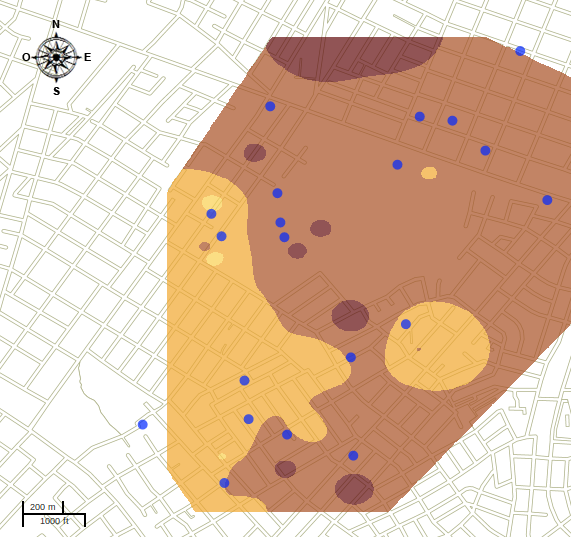
\includegraphics[width=\textwidth]{capitulo-6/graphics/raster/temp-20-38.png}
            \caption{\label{fig:niveles-infestacion-20-d}Día número 39 de simulación.}
    \end{subfigure}

    \caption{\label{fig:niveles-infestacion-20} Mapas de interpolación de la población correspondientes a los días 1, 29, 36 y 39 de simulación a 15 \textcelsius, y la distribución de las hembras adultas (puntos en azul). }
\end{figure}
